\documentclass[a4paper]{article}
\usepackage{times}
\usepackage[utf8]{inputenc}
\usepackage{selinput}
\usepackage{upquote}
\usepackage[margin=2cm, rmargin=4cm, tmargin=3cm]{geometry}
\usepackage{tcolorbox}
\usepackage{xspace}
\usepackage[french]{babel}
\usepackage{url}
\usepackage{hyperref}
\usepackage{fontawesome5}
\usepackage{marginnote}
\usepackage{ulem}
\usepackage{tcolorbox}
\usepackage{graphicx}
%\usepackage[top=Bcm, bottom=Hcm, outer=Ccm, inner=Acm, heightrounded, marginparwidth=Ecm, marginparsep=Dcm]{geometry}


\newtcolorbox{Example}[1]{colback=white,left=20pt,colframe=slideblue,fonttitle=\bfseries,title=#1}
\newtcolorbox{Solutions}[1]{colback=white,left=20pt,colframe=green,fonttitle=\bfseries,title=#1}
\newtcolorbox{Conseils}[1]{colback=white,left=20pt,colframe=slideblue,fonttitle=\bfseries,title=#1}
\newtcolorbox{Warning}[1]{colback=white,left=20pt,colframe=warning,fonttitle=\bfseries,title=#1}

\setlength\parindent{0pt}

  %Exercice environment
  \newcounter{exercice}
  \newenvironment{Exercice}[1][]
  {
  \par
  \stepcounter{exercice}\textbf{Question \arabic{exercice}:} (\faClock \enskip \textit{#1})
  }
  {\bigskip}
  

% Title
\newcommand{\titre}{\begin{center}
  \section*{Algorithmes et Pensée Computationnelle}
\end{center}}
\newcommand{\cours}[1]
{\begin{center} 
  \textit{#1}\\
\end{center}
  }


\newcommand{\exemple}[1]{\newline~\textbf{Exemple :} #1}
%\newcommand{\attention}[1]{\newline\faExclamationTriangle~\textbf{Attention :} #1}

% Documentation url (escape \# in the TP document)
\newcommand{\documentation}[1]{\faBookOpen~Documentation : \href{#1}{#1}}

% Clef API
\newcommand{\apikey}[1]{\faKey~Clé API : \lstinline{#1}}
\newcommand{\apiendpoint}[1]{\faGlobe~Url de base de l'API \href{#1}{#1}}

%Listing Python style
\usepackage{color}
\definecolor{slideblue}{RGB}{33,131,189}
\definecolor{green}{RGB}{0,190,100}
\definecolor{blue}{RGB}{121,142,213}
\definecolor{grey}{RGB}{120,120,120}
\definecolor{warning}{RGB}{235,186,1}

\usepackage{listings}
\lstdefinelanguage{texte}{
    keywordstyle=\color{black},
    numbers=none,
    frame=none,
    literate=
           {é}{{\'e}}1
           {è}{{\`e}}1
           {ê}{{\^e}}1
           {à}{{\`a}}1
           {â}{{\^a}}1
           {ù}{{\`u}}1
           {ü}{{\"u}}1
           {î}{{\^i}}1
           {ï}{{\"i}}1
           {ë}{{\"e}}1
           {Ç}{{\,C}}1
           {ç}{{\,c}}1,
    columns=fullflexible,keepspaces,
	breaklines=true,
	breakatwhitespace=true,
}
\lstset{
    language=Python,
	basicstyle=\bfseries\footnotesize,
	breaklines=true,
	breakatwhitespace=true,
	commentstyle=\color{grey},
	stringstyle=\color{slideblue},
  keywordstyle=\color{slideblue},
	morekeywords={with, as, True, False, Float, join, None, main, argparse, self, sort, __eq__, __add__, __ne__, __radd__, __del__, __ge__, __gt__, split, os, endswith, is_file, scandir, @classmethod},
	deletekeywords={id},
	showspaces=false,
	showstringspaces=false,
	columns=fullflexible,keepspaces,
	literate=
           {é}{{\'e}}1
           {è}{{\`e}}1
           {ê}{{\^e}}1
           {à}{{\`a}}1
           {â}{{\^a}}1
           {ù}{{\`u}}1
           {ü}{{\"u}}1
           {î}{{\^i}}1
           {ï}{{\"i}}1
           {ë}{{\"e}}1
           {Ç}{{\,C}}1
           {ç}{{\,c}}1,
    numbers=left,
}

\newtcbox{\mybox}{nobeforeafter,colframe=white,colback=slideblue,boxrule=0.5pt,arc=1.5pt, boxsep=0pt,left=2pt,right=2pt,top=2pt,bottom=2pt,tcbox raise base}
\newcommand{\projet}{\mybox{\textcolor{white}{\small projet}}\xspace}
\newcommand{\optionnel}{\mybox{\textcolor{white}{\small Optionnel}}\xspace}
\newcommand{\advanced}{\mybox{\textcolor{white}{\small Pour aller plus loin}}\xspace}
\newcommand{\auto}{\mybox{\textcolor{white}{\small Auto-évaluation}}\xspace}


\usepackage{environ}
\newif\ifShowSolution
\NewEnviron{solution}{
  \ifShowSolution
	\begin{Solutions}{\faTerminal \enskip Solution}
		\BODY
	\end{Solutions}
  \fi}


  \usepackage{environ}
  \newif\ifShowConseil
  \NewEnviron{conseil}{
    \ifShowConseil
    \begin{Conseils}{\faLightbulb \quad Conseil}
      \BODY
    \end{Conseils}

    \fi}

    \usepackage{environ}
  \newif\ifShowWarning
  \NewEnviron{attention}{
    \ifShowWarning
    \begin{Warning}{\faExclamationTriangle \quad Attention}
      \BODY
    \end{Warning}

    \fi}
  

%\newcommand{\Conseil}[1]{\ifShowIndice\ \newline\faLightbulb[regular]~#1\fi}


\usepackage{array}
\newcolumntype{C}[1]{>{\centering\let\newline\\\arraybackslash\hspace{0pt}}m{#1}}

\begin{document}
% Change the following values to true to show the solutions or/and the hints
\ShowSolutiontrue
\ShowConseiltrue
\titre
\cours{Programmation orientée objet}

Le code présenté dans les énoncés se trouve sur Moodle, dans le dossier \lstinline{Ressources}.

\section{Conception de classes pour coder des weighted graphs}

\subsection{Partie 1}
Ici on cherche à pousser votre réflexion sur le processus de conception de classes pour implémenter un concept existant en dehors de la programmation.
Pour cela il faut se placer du point de vue de l'utilisateur pour savoir ce dont il aurait besoin. 
Il faut aussi savoir de quoi est constitué le concept que l'on cherche à implémenter. C'est à dire, pour utiliser une analogie, les différentes briques qui sont utilisées pour construire le mur qui est votre objet final.

Cette partie de l'exercice a pour but de poser des questions théoriques qui sont une aide pour comprendre la logique de conception.

\begin{Exercice}[Durée 15 minutes] Exercice 1\\
    \begin{enumerate}
        \item Quels sont les 3 composants d'un weighted graph ?
        \item Combien de classes sont nécéssaires pour représenter tous les composants du graph et le graph lui même ?
        \item Sachant que vous avez une classe qui représente les arêtes et que les sommets sont représentés par des chaînes de caractères. Déterminer quels sont les attributs de la class graph.
        \item Maintenant que vous avec le schéma général de votre classe graph, il faut déterminer quelles méthodes sont nécéssaires au fonctionnement de cet objet.
        
        Il faut donc réfléchir sur les questions suivantes:
            \begin{enumerate}
            \item Est-ce que l'utilisateur aura besoin de modifier l'objet une fois celui-ci initialisé ?
            \item Est-ce que l'utilisateur aura besoin de vérifier l'état de l'objet ( existence d'attributs, vérification de valeurs...) ou de certaines parties de l'objet ?
            \item Est-il nécéssaire de définir des méthodes qui ne seront pas utiles pour l'utilisateur mais utiles pour éviter la redondance du code ?
            \end{enumerate}
    \end{enumerate}
    Une fois ces questions répondues, le schéma des méthodes nécessaires devient plus claire.
    
    Il reste enfin à traiter l'implémentation de tout cela. C'est à dire, comment coder la classe pour qu'elle soit fonctionnelle.
\begin{conseil}
   % Un conseil
   \begin{enumerate}
   \item Il faut décomposer ce qui constitue un graph. Revenir sur le cours de la semaine 7 sur moodle.
   \item Réfléchir aux différents objets du type les arêtes qui consituent un graph. Réflechir si ils ont besoin d'être représenté avec une classe ou est-ce que les types de "base" sont suffisants.
   \item Les attributs sont les briques qui constituent votre classe. Il faut donc poser les variables nécéssaires et leur type.
   \item Penser de la même manière que lorsque vous utilisez une application et critiquez (en bien ou en mal) les fonctionnalitées de celle-ci. Ici, il faut réfléchir à ce qu'une personne qui va utiliser votre "application" ( la classe) aurait besoin.
   \end{enumerate}
\end{conseil}
    
\begin{solution}
\textbf{Certaines questions n'ont pas qu'une réponse car il y a toujours plus d'une manière d'implémenter une classe. Voici une façon de répondre: }
    %\lstinputlisting{solutions/fichier.java}
    \begin{enumerate}
    \item \begin{enumerate}
          \item Les sommets.
          \item Les arêtes.
          \item Le poids de chaque arête.
          \end{enumerate}
    \item Il faut 2 classes ( ou 3 si on cherche à avoir plus d'informations dans les sommets):
        \begin{enumerate}
        \item Une classe Edges qui va représenter les arêtes.
        \item Une classe graph.
        \end{enumerate}
    \item La classe graph va avoir 2 attributs: un ensemble contenant les sommets et un autre ensemble contenant les arêtes de celui-ci.
    \item Les réponses à cette partie sont courtes mais assez essentielles pour savoir quelles méthodes coder:
        \begin{enumerate}
        \item Oui, l'utilisateur voudra sûrement rajouter des arêtes, des sommets ou potentiellement changer le poids d'une arête. Il faut donc lui laisser cette possibilité
        \item Les graphs sont souvent accompagnés par des algorithmes de recherche, par exemple l'algorithme de Kruskal pour les weighted graphs. Il est donc utile de pouvoir identifier si un sommet ou une arête sont des composants de l'instance.
        \item Certaines méthodes pourraient avoir un code très long si on ne ségmentarise pas leur contenu. Cela peut entraver la relecture de votre code par vous ou par un tiers. 
        
        De plus dans un cadre d'optimisation, il faut éviter un maximum la redondance du code. Il est donc de bonne pratique de définir des méthodes qui vont éviter cela dans une classe.
        \end{enumerate}
    \end{enumerate}
\end{solution}
\newpage
\end{Exercice}
\subsection{Partie 2}
Le code pour la classe Edges est fourni dans le dossier ressources sur moodle.
Utiliser le fichier Main.java dans le dossier ressources sur moodle pour effectuer des tests. Il devrait retourner:

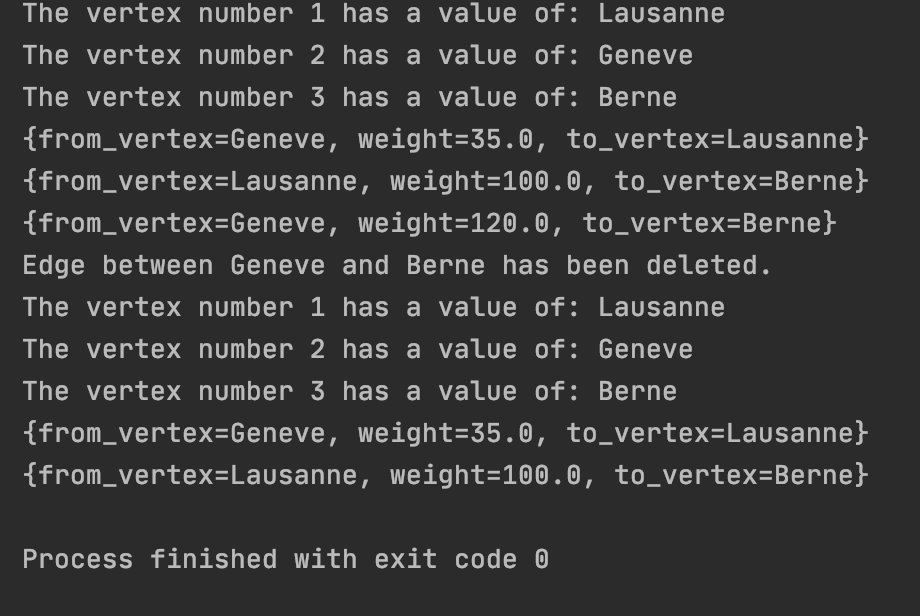
\includegraphics[]{sortie_juste.PNG}
\begin{Exercice}[Durée 20 minutes] Exercice 2\\
Voici une partie de la classe graph codée. Implémentez les méthodes "update_weight", "new_edge" et " "edge_exist".

\textbf{Java :}
         \lstinputlisting{graph_empty.java}
\endgroup
    \begin{enumerate}
        \item La méthode "update weight" doit prendre en paramètres: le sommet d'origine, le sommet d'arrivée ainsi que le poids d'une arête. Si cette arête existe alors elle change son poids. Sinon elle imprimera une phrase indiquant que cette arête n'existe pas.
        \item La méthode "edge exist" qui va prendre en paramètre le sommet d'origine et le sommet d'arrivée. Si cette arête est dans le graph alors la méthode ressort son poids, 0 sinon.
        \item La méthode "new edge" doit créer une instance de Edges et l'ajouter à l'ensemble edges si la connexion n'existe pas déjà. Si elle existe avec un autre poids mettre à jour le poids. Si elle existe de façon identique alors retournez la dans la console avec print. Enfin, si on est dans aucun des deux cas précédents utiliser la méthode "generate edge" qui vous est donnée pour créer et ajouter cette arête au graph. La méthode "new edge" aura comme paramètres: le sommet d'origine, le sommet d'arrivée, le poids.
    \end{enumerate}

    \begin{conseil}
    \begin{enumerate}
    \item Utiliser une boucle for pour parcourir toutes les arêtes dans le graph. Faire un test sur les attributs de Edges pour changer le poids.
    \item Il faut tester pour chaque arête ( itération) si elle  est égale à celle rentrée en paramètres.
    \item Il faut utiliser les méthodes " edge exist", " update edge" et " generate edge" pour écrire cette méthode. Il y a 4 tests à effectuer: 
        \begin{enumerate}
        \item Si l'arête existe.
        \item Si l'arête existante a le même poids que celui indiqué en paramètre de la méthode.
        \item Si l'arête existante n'a pas le même poids que celui indiqué en paramètre de la méthode.
        \item Utiliser le résultat de " edge exist" pour simplifier ces tests.
        \end{enumerate}
    \end{enumerate}
    \end{conseil}
    \begin{solution}
    \textbf{Java :}
         \lstinputlisting{Edges.java}
    \end{solution}
    \begin{solution}
    \textbf{Java :}
         \lstinputlisting{graph.java}
    \end{solution}
    \begin{solution}
    \textbf{Java :}
         \lstinputlisting{graph2.java}
    \end{solution}
    \end{Exercice}
\end{document}
